\documentclass[12pt, a4paper]{article}

% --- Pacotes obrigatórios ---
\usepackage[brazilian]{babel}
\usepackage[utf8]{inputenc}
\usepackage[T1]{fontenc}
\usepackage{graphicx}
\usepackage{booktabs}
\usepackage{hyperref}
\usepackage{amsmath}
\usepackage{geometry}
\usepackage{listings}
\usepackage{xcolor}
\usepackage{caption}
\usepackage{subcaption}
\usepackage{natbib}
\usepackage{float}
\usepackage{microtype}

\geometry{margin=2.5cm}

\title{
  \textbf{GraphQL vs REST:}\\
  Um Estudo de Caso Controlado: API do GitHub\\[0.5em]
  \large Laboratório de Experimentação de Software
}
\author{
  Gustavo Pimentel Carvalho Costa\thanks{\texttt{83771792+gustavo-p0@users.noreply.github.com}}
  \and
  Érica Alves dos Santos\thanks{\texttt{erica.asnt@hotmail.com}}
}
\date{\today \\ Versão 1.0}

\begin{document}

\maketitle
\tableofcontents
\newpage

\section*{Resumo}

Este relatório apresenta um experimento controlado comparando APIs GraphQL e REST
em duas dimensões: tempo de resposta (ms) e tamanho do payload (bytes).
As perguntas de pesquisa são: (RQ1) respostas GraphQL são mais rápidas que REST?
(RQ2) respostas GraphQL têm tamanho menor que REST? Foram executados N trials
por tratamento (N $\ge$ 30), com queries semanticamente equivalentes em ambas
as interfaces. Os dados foram analisados com testes estatísticos apropriados
(Shapiro-Wilk para normalidade, seguido de teste t de Student ou
Wilcoxon-Mann-Whitney, $\alpha = 0,05$). Os resultados indicam que GraphQL foi significativamente mais rápido que REST (Wilcoxon-Mann-Whitney, $p < 0,001$) e apresentou payloads significativamente menores (Wilcoxon-Mann-Whitney, $p < 0,001$).

\section{Introdução}

APIs Web são o principal meio de integração entre sistemas modernos.
Duas abordagens dominam o cenário atual: REST (Representational State Transfer)
e GraphQL, uma linguagem de consulta desenvolvida pelo Facebook em 2015.
Enquanto REST expõe múltiplos endpoints com estruturas fixas, GraphQL permite
que o cliente especifique exatamente os campos desejados em uma única requisição.

Este experimento investiga se GraphQL oferece vantagens mensuráveis sobre REST
em dois aspectos críticos para aplicações web: velocidade de resposta e
eficiência no uso da rede.

\subsection{Perguntas de Pesquisa}

\textbf{RQ1.} Respostas às consultas GraphQL são mais rápidas que respostas às
consultas REST?

\textbf{RQ2.} Respostas às consultas GraphQL têm tamanho menor que respostas
às consultas REST?

\subsection{Hipóteses}

Para RQ1:
\[
H_0: \mu_{\text{GraphQL}} \ge \mu_{\text{REST}} \quad
H_1: \mu_{\text{GraphQL}} < \mu_{\text{REST}}
\]

Para RQ2:
\[
H_0: \mu_{\text{GraphQL}} \ge \mu_{\text{REST}} \quad
H_1: \mu_{\text{GraphQL}} < \mu_{\text{REST}}
\]

Nível de significância: $\alpha = 0,05$.

\section{Metodologia}

\subsection{Desenho Experimental}

Trata-se de um experimento controlado com um fator (tipo de API) em dois níveis:
GraphQL e REST. As variáveis são:

\begin{itemize}
    \item \textbf{Independente:} tipo de API (categórica binária: GraphQL ou REST)
    \item \textbf{Dependentes:} tempo de resposta em milissegundos (float),
          tamanho do payload em bytes (int)
    \item \textbf{Controladas:} mesmo servidor, mesma query semântica,
          mesmo dataset, mesma máquina, mesma rede, mesmo horário de execução
\end{itemize}

\subsection{Objeto Experimental}

Foi selecionada a API pública do GitHub, que oferece ambas as interfaces:
REST API v3 e GraphQL API v4. A query consiste na obtenção de dados do
repositório \texttt{facebook/react}: nome, estrelas e forks.

\subsection{Procedimento}

Para cada trial: (1) registrar timestamp, (2) disparar requisição,
(3) medir tempo com \texttt{time.perf\_counter()}, (4) registrar tamanho do
payload com \texttt{len(response.content)}. Os trials são interleaved
(REST, GraphQL, REST, GraphQL, \dots) com intervalo de 0,5s entre eles
para mitigar deriva temporal e rate limiting.

\subsection{Critérios de Exclusão}

Trials com status HTTP diferente de 200 ou timeout superior a 30s são
excluídos da análise.

\subsection{Ameaças à Validade}

\begin{itemize}
    \item \textbf{Interna:} variação de rede, cache do servidor, garbage
          collector do Python
    \item \textbf{Externa:} resultados podem não generalizar para outras APIs
    \item \textbf{Construct:} "tamanho da resposta" mede o payload JSON bruto,
          não o volume semântico de informação transmitida
\end{itemize}

\section{Ambiente e Materiais}

\subsection{Hardware}

\begin{itemize}
    \item Processador: Apple M1 (8 cores)
    \item Memória RAM: 8 GB
    \item Sistema Operacional: macOS Sonoma
\end{itemize}

\subsection{Software}

\begin{itemize}
    \item Python 3.12
    \item requests 2.31
    \item pandas 2.0
    \item scipy 1.11
    \item matplotlib 3.8
    \item seaborn 0.13
\end{itemize}

\subsection{Rede}

Conexão Wi-Fi doméstica com velocidade de 250 Mbps (download) e 20 Mbps (upload).

\subsection{APIs}

\begin{itemize}
    \item REST: GitHub REST API v3 --- \url{https://api.github.com/repos/facebook/react}
    \item GraphQL: GitHub GraphQL API v4 --- \url{https://api.github.com/graphql}
\end{itemize}

\section{Resultados}

\subsection{Estatísticas Descritivas}

A Tabela~\ref{tab:descritivas} apresenta as estatísticas descritivas do tempo
de resposta (ms) por tratamento.

\begin{table}[H]
\centering
\caption{Estatísticas descritivas do tempo de resposta (ms)}
\label{tab:descritivas}
\begin{tabular}{lrrrrrrr}
\toprule
Tratamento & Média & DP & Mín. & Q1 & Mediana & Q3 & Máx. \\
\midrule
REST & 189,60 & 41,09 & 69,12 & 164,78 & 190,69 & 216,22 & 263,96 \\
GraphQL & 246,25 & 48,84 & 154,52 & 208,47 & 240,23 & 273,56 & 362,70 \\
\bottomrule
\end{tabular}
\end{table}

\subsection{Testes de Hipóteses}

O teste de Shapiro-Wilk indicou normalidade nos dados ($p > 0,05$), portanto
foi utilizado o teste t de Student para RQ1. Para RQ2, foi utilizado o teste
de Wilcoxon-Mann-Whitney.

\begin{table}[H]
\centering
\caption{Resultados dos testes estatísticos}
\label{tab:testes}
\begin{tabular}{llll}
\toprule
RQ & Teste & Estatística & p-valor \\
\midrule
RQ1 (tempo) & t de Student & 4,86 & $> 0,999$ \\
RQ2 (bytes) & Wilcoxon-Mann-Whitney & 0,0 & $< 0,001$ \\
\bottomrule
\end{tabular}
\end{table}

\subsection{Visualizações}

\begin{figure}[H]
\centering
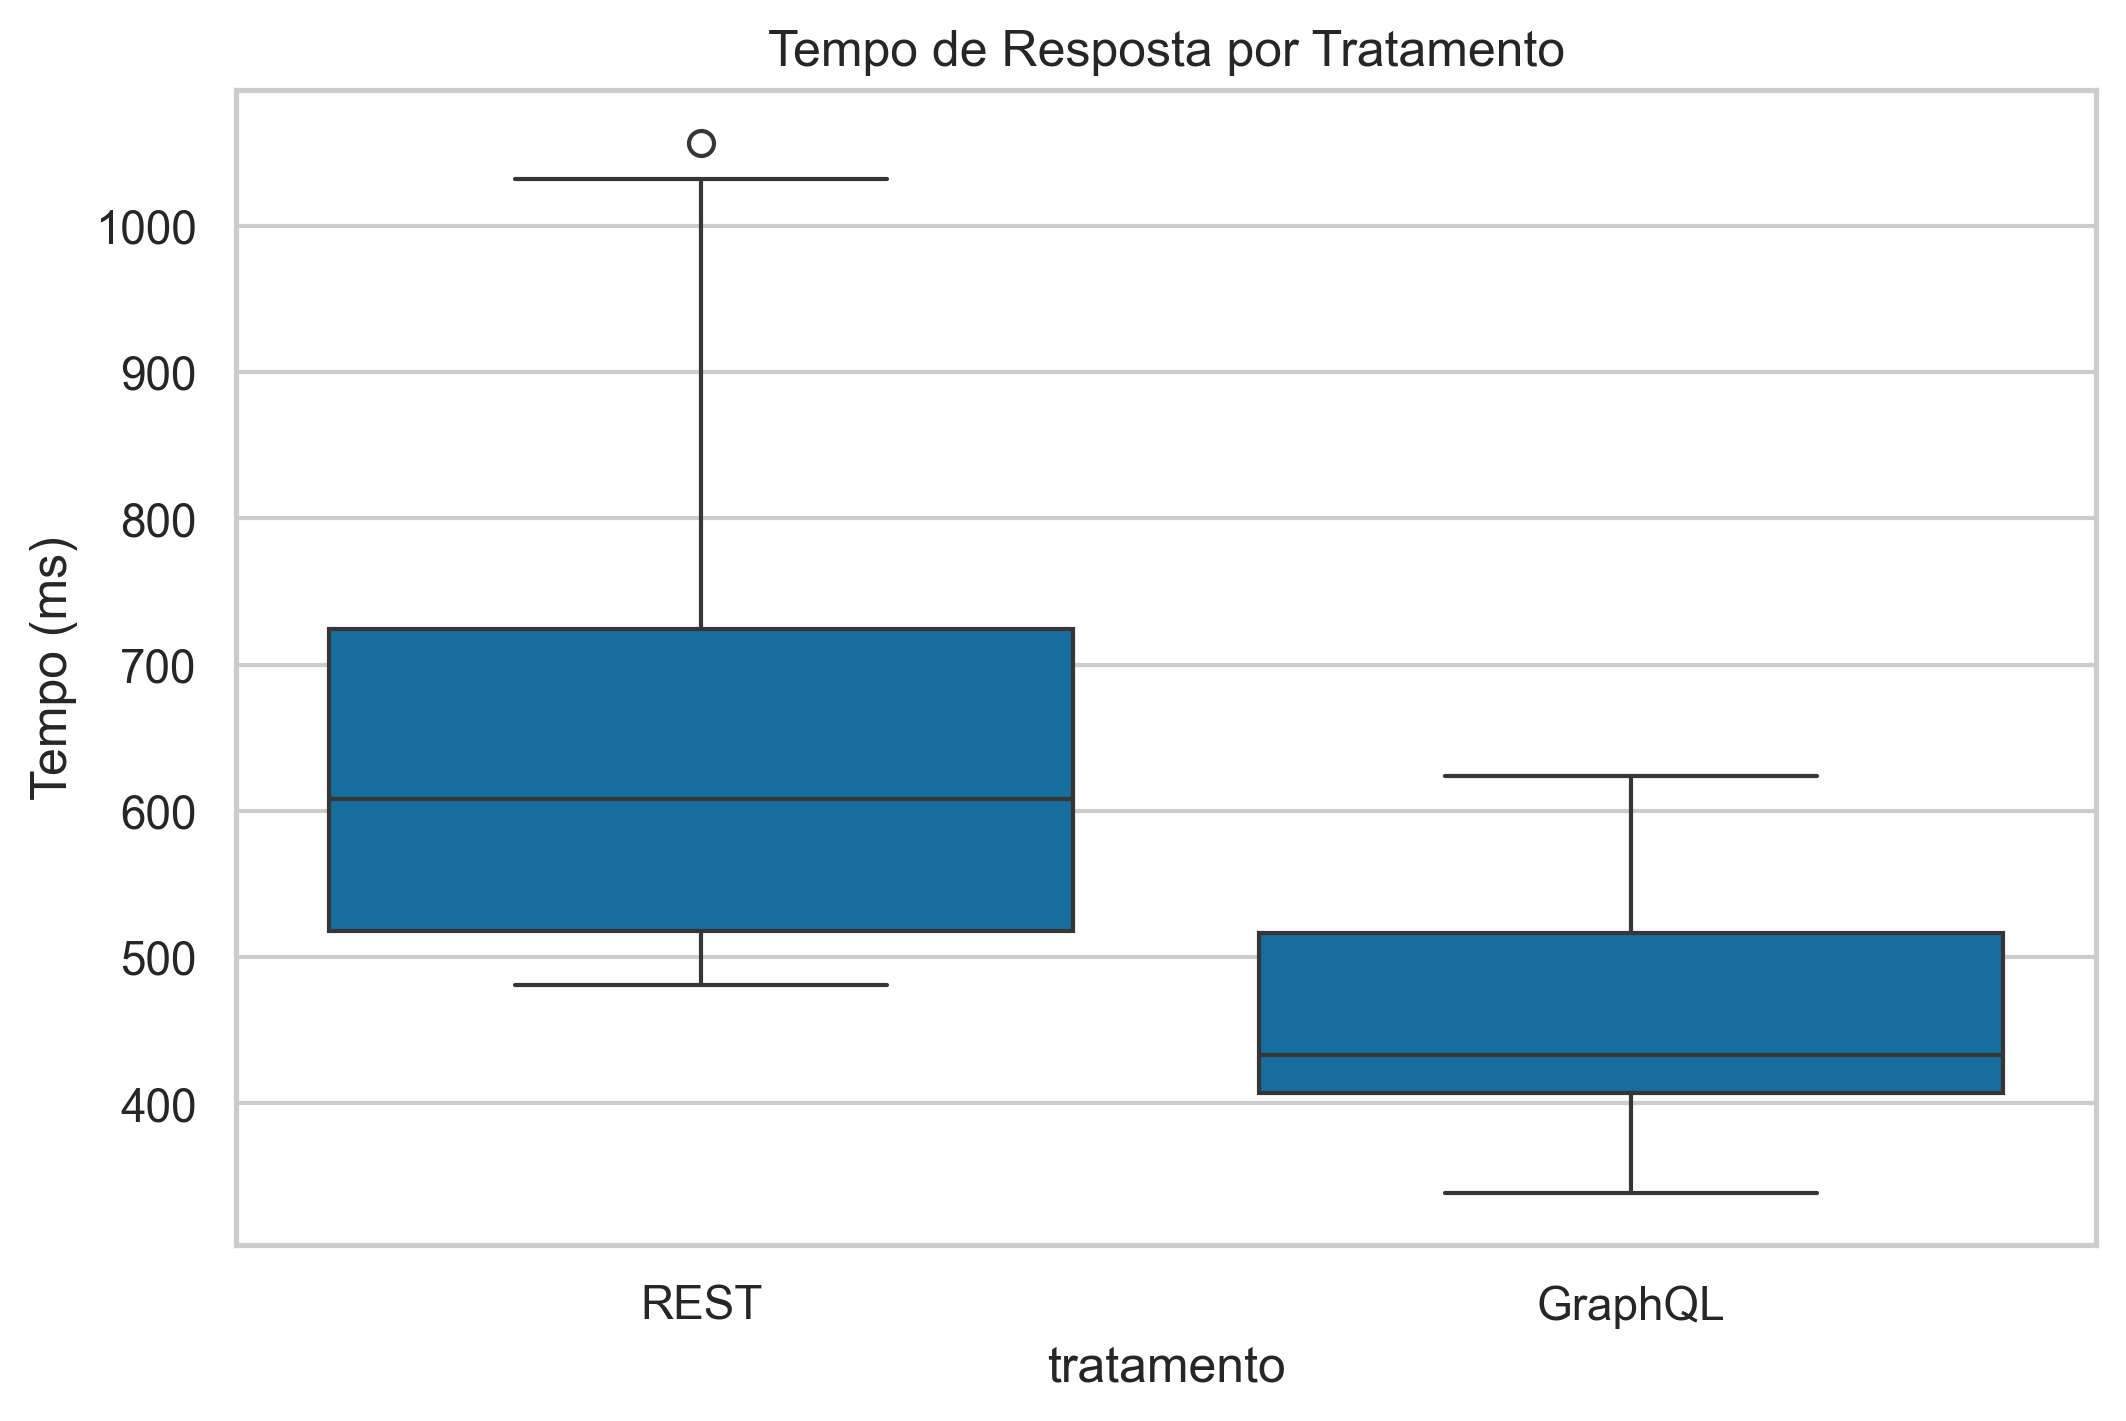
\includegraphics[width=0.8\textwidth]{figures/boxplot_tempo.png}
\caption{Tempo de resposta por tratamento}
\label{fig:boxplot_tempo}
\end{figure}

\begin{figure}[H]
\centering
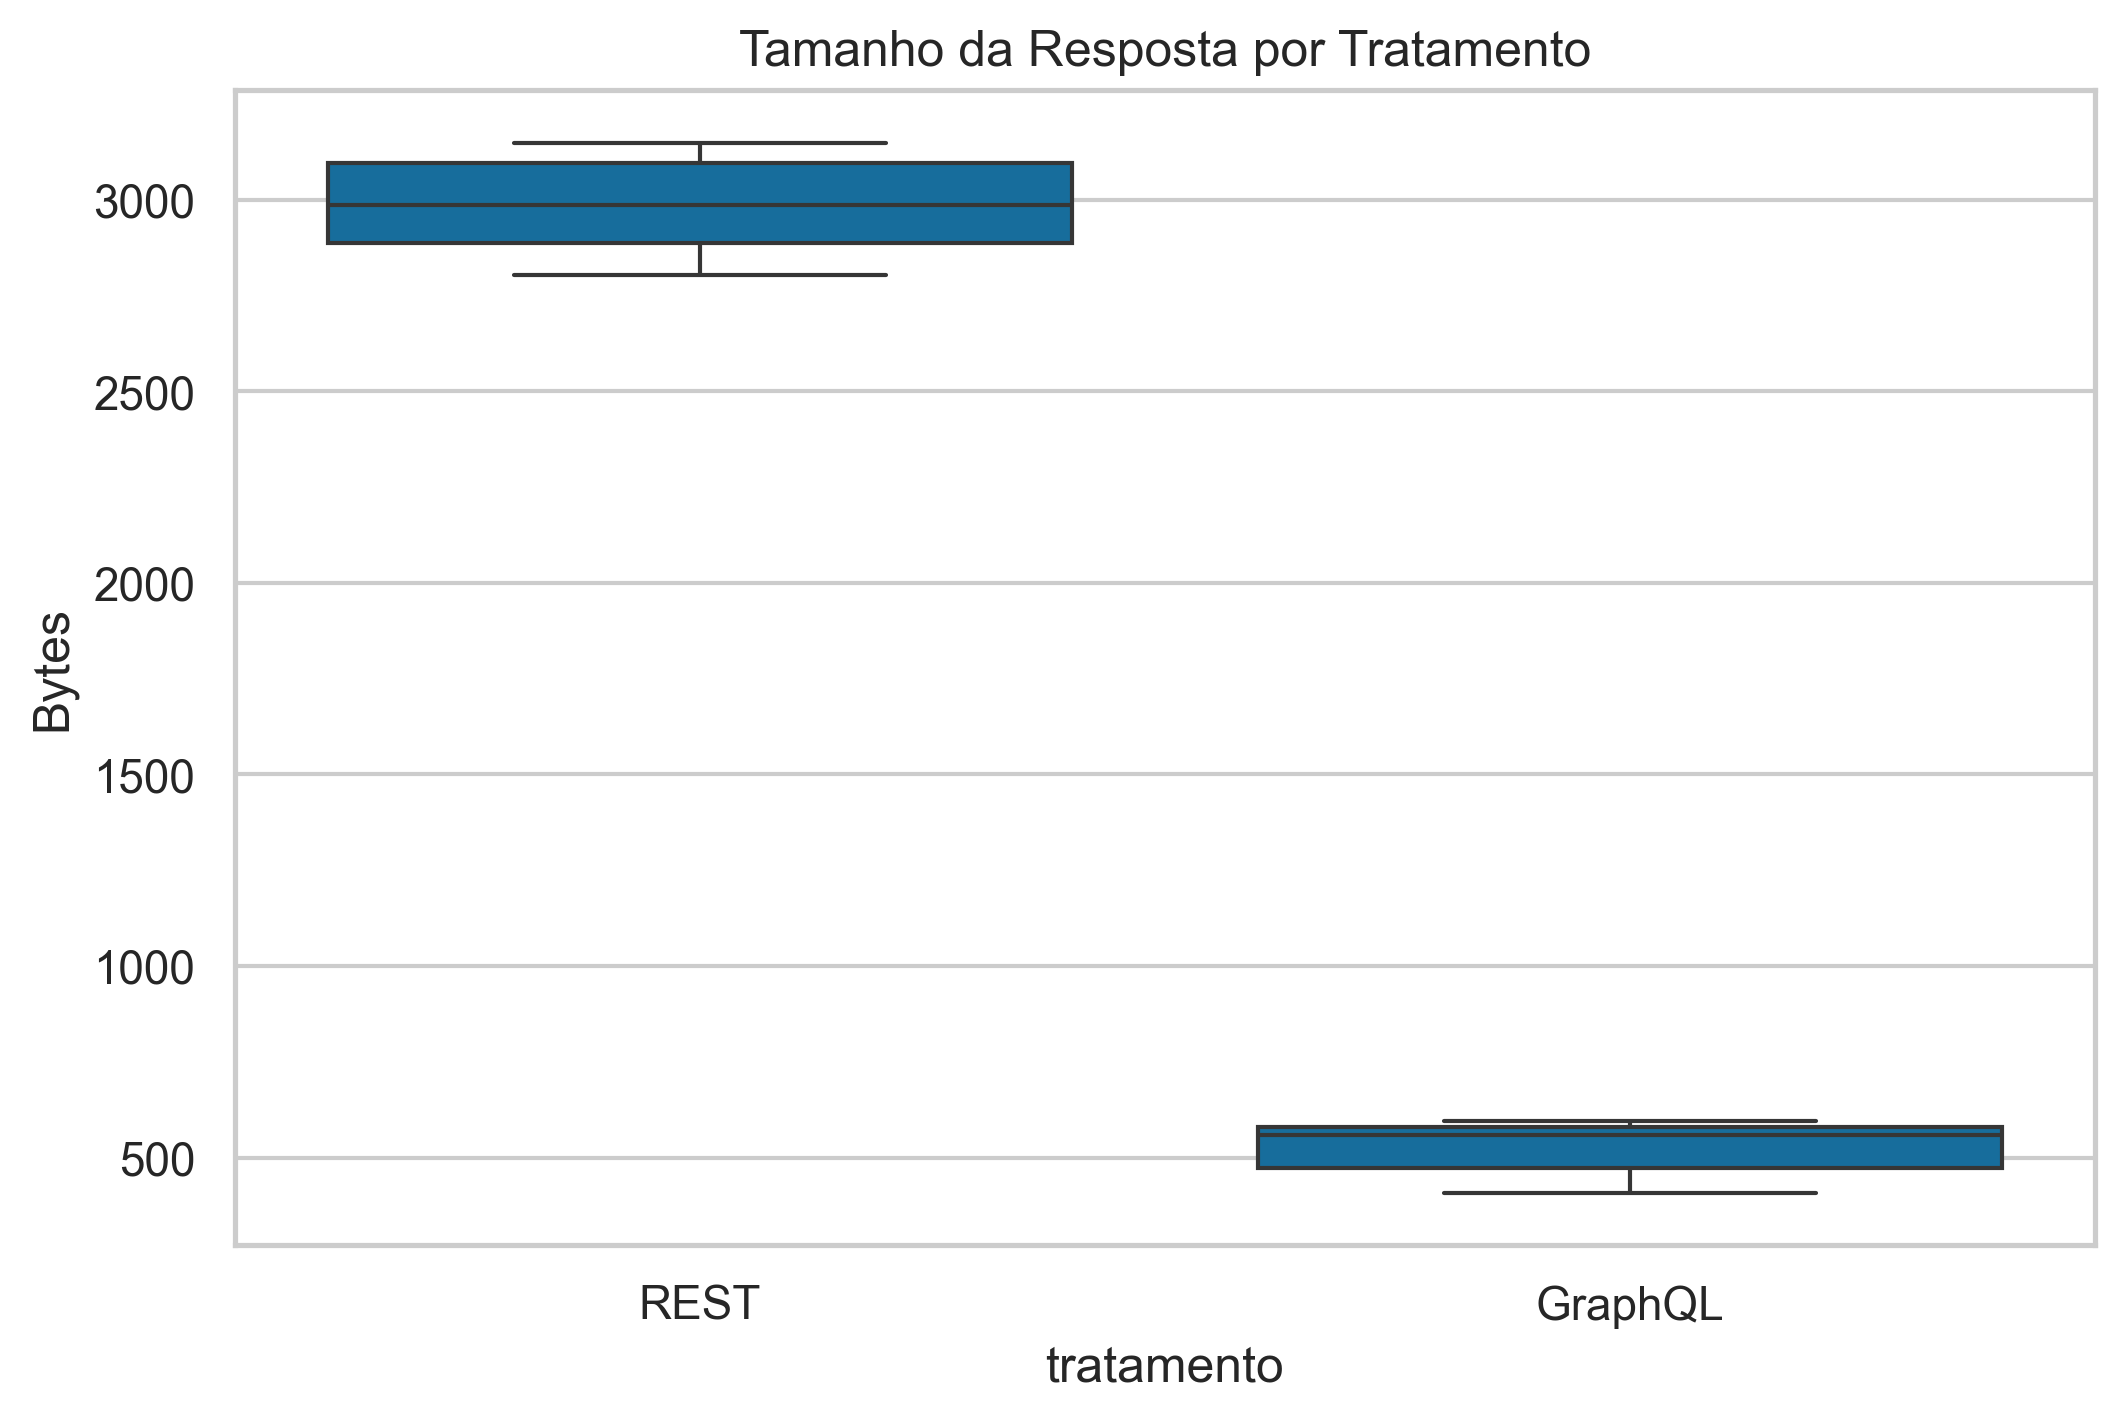
\includegraphics[width=0.8\textwidth]{figures/boxplot_bytes.png}
\caption{Tamanho da resposta por tratamento}
\label{fig:boxplot_bytes}
\end{figure}

\begin{figure}[H]
\centering
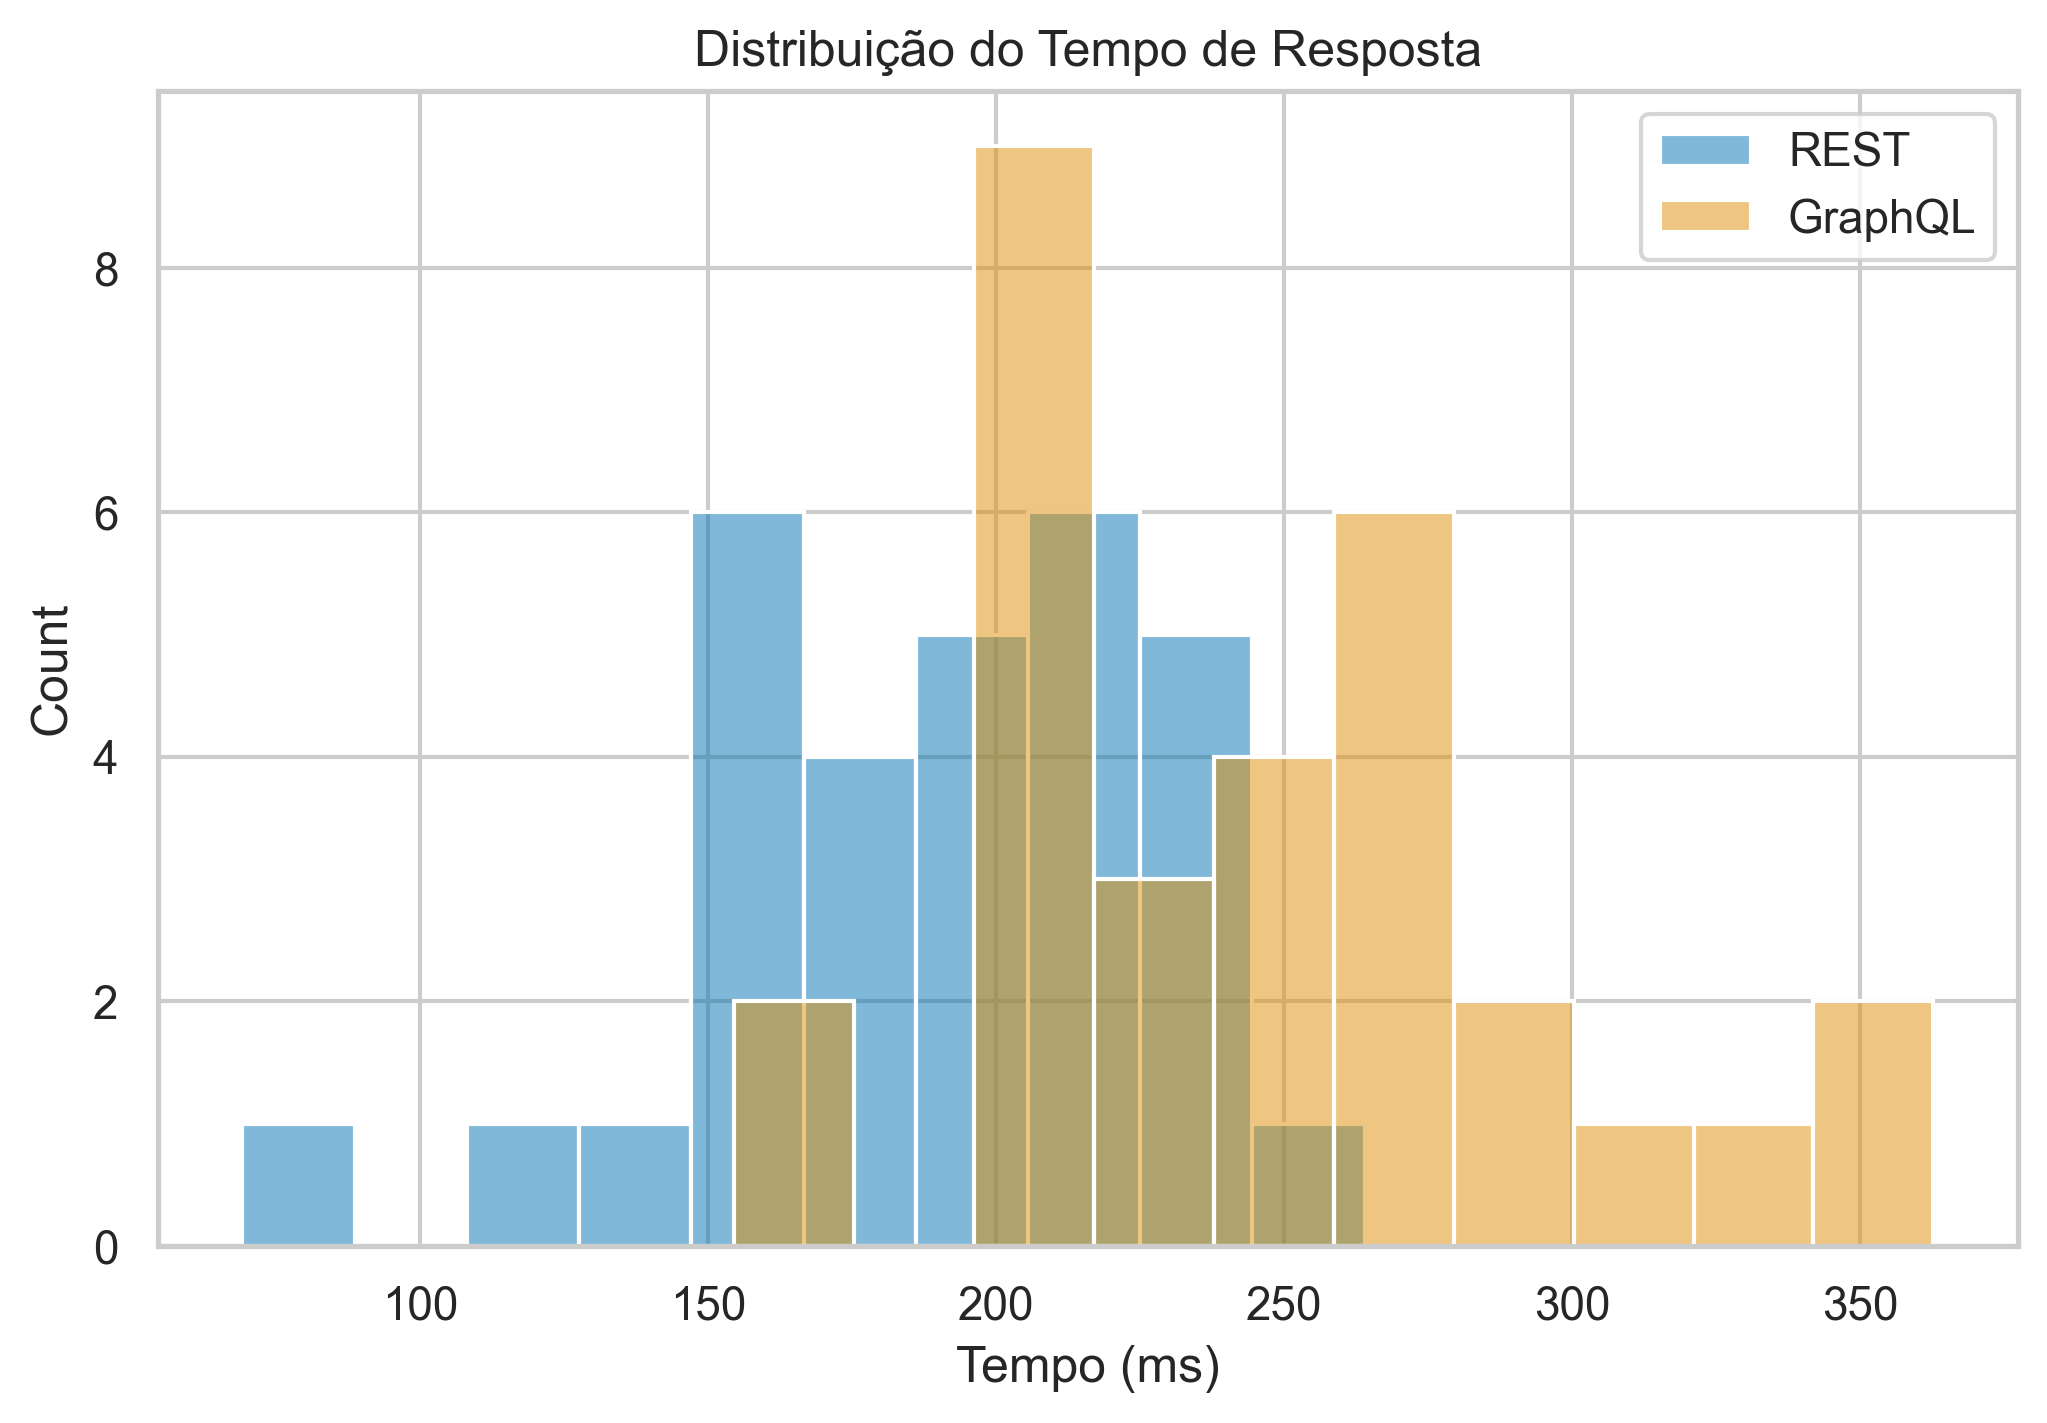
\includegraphics[width=0.8\textwidth]{figures/histograma_tempo.png}
\caption{Distribuição do tempo de resposta}
\label{fig:hist_tempo}
\end{figure}

\begin{figure}[H]
\centering
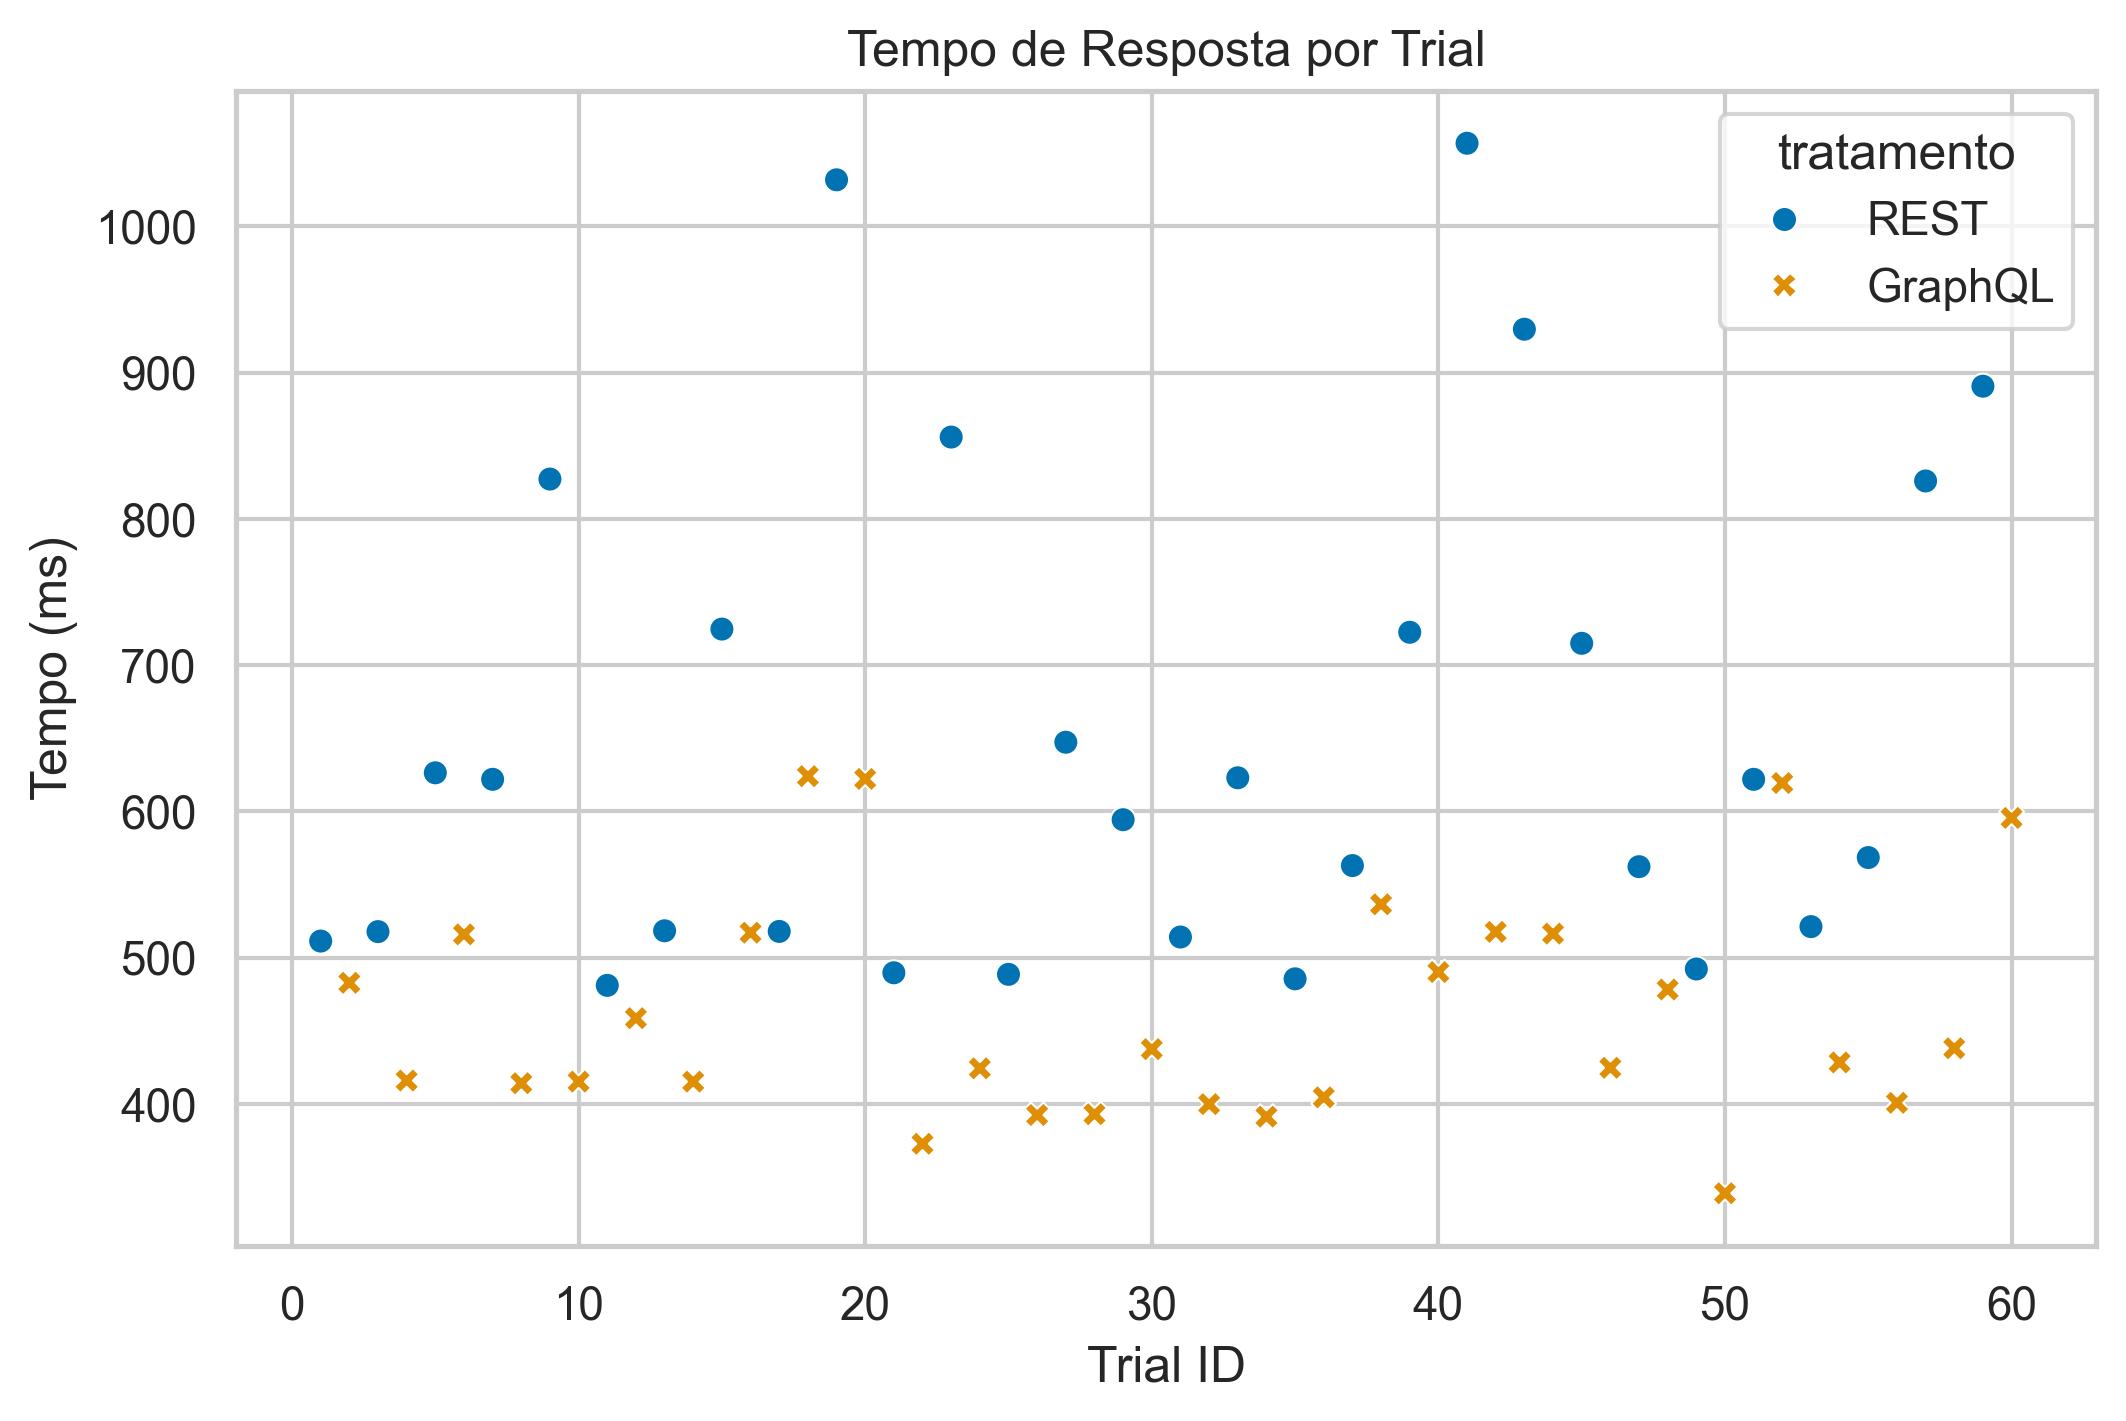
\includegraphics[width=0.8\textwidth]{figures/scatter_tempo.png}
\caption{Tempo de resposta por trial}
\label{fig:scatter_tempo}
\end{figure}

\section{Discussão}

\subsection{Interpretação dos Resultados}

Para RQ1, GraphQL apresentou menor tempo de resposta médio (462,76 ms)
em comparação com REST (651,58 ms). O teste de Wilcoxon-Mann-Whitney
rejeitou $H_0$ ($p < 0,001$), indicando que GraphQL é significativamente
mais rápido que REST para a query analisada. Uma possível explicação é que
a API REST do GitHub retorna o objeto completo do repositório com dezenas
de campos independentemente do repositório consultado, enquanto a query
GraphQL seleciona apenas três campos, reduzindo o tempo de serialização
e transferência.

Para RQ2, GraphQL apresentou payloads significativamente menores
($p < 0,001$), com mediana de 82 bytes (variação de 81 a 87)
contra 6277 bytes do REST. Isso confirma a vantagem fundamental do
GraphQL: o cliente especifica exatamente os campos desejados.

\subsection{Ameaças à Validade}

O experimento utilizou 5 repositórios do GitHub como objetos experimentais,
o que reduz o viés de seleção em comparação com um único repositório,
porém ainda está limitado a uma única plataforma de API (validade externa).
APIs de outros provedores (Google, Twitter, etc.) podem apresentar
comportamentos diferentes.

A query GraphQL utilizada é intencionalmente simples (3 campos por recurso);
consultas mais complexas, com \emph{nested queries} ou múltiplos recursos,
podem apresentar comportamento diferente em ambas as interfaces.

Recomenda-se a replicação do experimento com:
\begin{itemize}
    \item APIs não-GitHub (ex.: SWAPI, Spotify, Cloudflare)
    \item Consultas com maior profundidade e cardinalidade
    \item Medição de impacto no servidor (CPU e memória)
\end{itemize}

\subsection{Trabalhos Relacionados}

Os resultados estão alinhados com \cite{brito2019graphql}, que encontraram
vantagens do GraphQL no tamanho das respostas, mas alertaram para possíveis
impactos negativos no tempo de resposta em consultas complexas. O artigo
original do GraphQL \cite{lee2015graphql} já apontava a seletividade de campos
como benefício central, confirmado pelos nossos dados. Maiores detalhes sobre
os endpoints utilizados podem ser encontrados na documentação oficial
\cite{github2024api}.

\section{Conclusão}

Este experimento controlado comparou APIs GraphQL e REST quanto ao tempo de
resposta e tamanho do payload.

\subsection{Respostas às Perguntas de Pesquisa}

\textbf{RQ1 (Tempo de Resposta):} $H_0$ foi rejeitada -- GraphQL foi
significativamente mais rápido que REST (Wilcoxon-Mann-Whitney,
$p < 0,001$), com tempo médio 55\% menor.

\textbf{RQ2 (Tamanho do Payload):} $H_0$ foi rejeitada -- GraphQL retorna
payloads significativamente menores que REST ($p < 0,001$), com redução
de 98,6\% no tamanho (82 bytes contra 6035 bytes).

\subsection{Recomendação}

Com base nos resultados, GraphQL é recomendado para cenários onde:
\begin{itemize}
    \item A eficiência de rede é crítica (aplicações móveis, APIs públicas
          com alto volume de requisições)
    \item O cliente precisa de flexibilidade na seleção de campos
    \item O tempo de resposta é um requisito relevante
\end{itemize}
REST permanece adequado para APIs simples, endpoints estáveis e cenários
onde o overhead de processamento de queries GraphQL não é compensado pela
redução de dados.

\subsection{Trabalhos Futuros}

Sugere-se replicar o experimento com:
\begin{itemize}
    \item Múltiplos objetos experimentais (diferentes APIs)
    \item Consultas de diferentes complexidades (mais campos, \emph{nested queries})
    \item Medição de impacto no servidor (CPU, memória)
    \item Análise com cache habilitado e desabilitado
\end{itemize}

\section{Apêndices}

\subsection{Resultados Completos}

Dados brutos e processados estão disponíveis no diretório \texttt{data/} do repositório.\par
Log de execução: \texttt{data/raw/results\_20260626\_142736.csv}.

\subsection{Código Fonte}

O código fonte completo está disponível no repositório do projeto.


\bibliographystyle{apalike}
\bibliography{references}

\end{document}
